\section{Systemmodelle}

\subsection{Anwendungsfalldiagramme}

\subsubsection*{Kartenansicht}
\noindent\makebox[\textwidth]{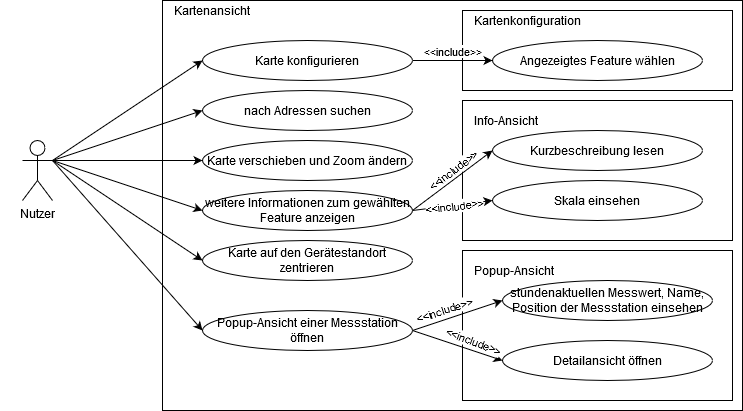
\includegraphics[width=\textwidth]{Anwendungsfalldiagramm_Kartenansicht.png}}

\subsubsection*{Detailansicht}
\noindent\makebox[\textwidth]{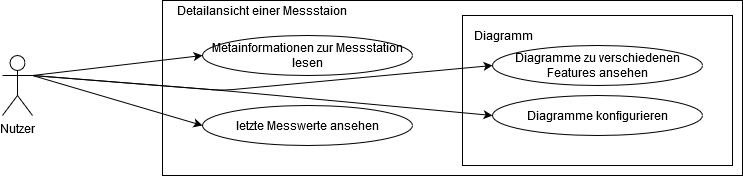
\includegraphics[width=\textwidth]{Anwendungsfalldiagramm_Detailansicht.png}}
\newpage

\subsection{Architekturdiagramm}

\noindent\makebox[\textwidth]{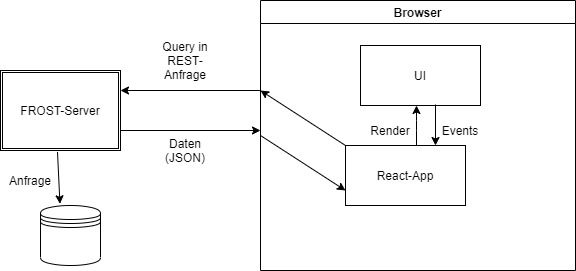
\includegraphics[width=\textwidth]{Architekturdiagramm.jpg}}
\subsection{Ablaufdiagramm}

\noindent\makebox[\textwidth]{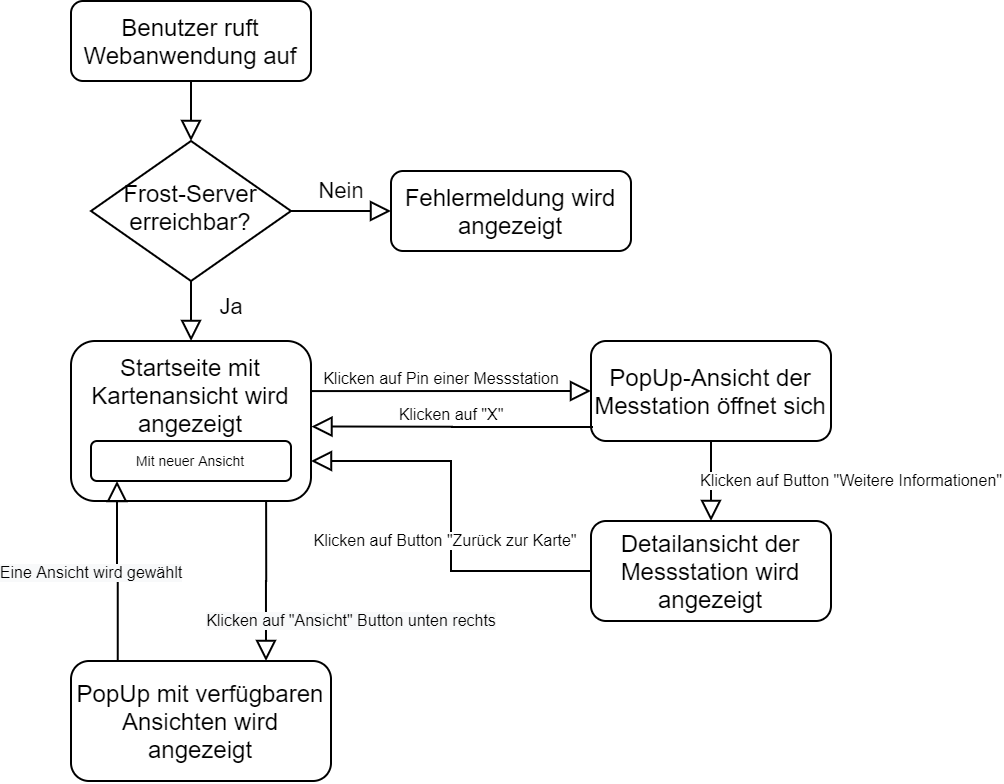
\includegraphics[width=\textwidth]{Ablaufdiagramm.png}}

\subsection{Szenarios}

\subsubsection*{Szenario 1: Ansicht, der studenaktuellen Feinstaubwerte (PM 10) am Smartphone}
\textbf{Nutzer:} Nutzer mit grundlegenden IT-Kenntnissen der schon einmal ähnliche Anwendungen bedient hat (z.B. Google Maps) 
und somit intuitiv die Karte bedienen kann. Des Weiteren hat er jedoch wenig Kenntnisse über Feinstaubwerte und benötigt somit 
eine Einordnung und Erklärung der \glspl{Messwert}.

\textbf{Beschreibung:} Der Nutzer interessiert sich für die aktuellen Feinstaubwerte in seiner Stadt.

\textbf{Konkreter Ablauf:}
Der Nutzer öffnet die \gls{Webanwendung}, indem er die URL der \gls{Webanwendung} in seinen Smartphone Browser eingibt und bestätigt. Daraufhin öffnet 
sich die Kartenansicht der Anwendung. Dort sind die \glspl{Station} als Punkt eingetragen. Über einen Button in der rechten unteren 
Ecke ruft der Nutzer das Konfigurationsmenü der Karte auf. Dort Klickt er auf PM 10 (Feinstaub). Daraufhin werden nur die 
\glspl{Station} als Punkt auf der Karte angezeigt, die das \gls{Feature} PM10 messen und sie werden, aufgrund ihres zuletzt 
gemessenen PM10 Wertes eingefärbt. Desto grüner ein Punkt, desto niedriger der Wert. Desto roter ein Punkt, desto höher ein Wert. 
Die Farbskala wird in der linke unteren Ecke angezeigt.
Um einen \gls{Messwert} in Zahlenform einer \gls{Station} anzuzeigen, klickt der Nutzer auf einen Punkt. Daraufhin öffnet am 
unteren Bildschirmrand eine Popup-Ansicht, in der der Name der \gls{Station}, die Position und der PM10 Wert angezeigt wird. 
Außerdem wird eine Warnung angezeigt, wenn der \gls{Messwert} einen Grenzwert überschritten hat.
\newpage

\subsubsection*{Szenario 2: Ansicht der Diagramme einer spezifischen Messstation am Computer}
\textbf{Nutzer:} Nutzer mit grundlegenden IT-Kenntnissen der schon einmal ähnliche Anwendungen bedient hat (z.B. Google Maps) 
und somit intuitiv die Karte bedienen kann. Er hat sich schon häufiger über Luftqualität informiert und ist an konkreten 
\glspl{Messwert}n und deren zeitlicher Entwicklung interessiert.

\textbf{Beschreibung:} Der Nutzer möchte Diagramme einer \gls{Station} einsehen.

\textbf{Konkreter Ablauf:} Der Nutzer öffnet die \gls{Webanwendung}, indem er die URL der \gls{Webanwendung} in in den Browser seines Computer eintippt 
und bestätigt. Daraufhin öffnet sich die Kartenansicht der \gls{Webanwendung}. Über das Suchfeld in der linken oberen Ecke gibt 
er eine Adresse ein oder klickt auf den Button zur Standortbestimmung. Daraufhin zentriert sich die Karte auf den genwünschten Ort. 
Der Nutzer klickt nun auf einen Punkt in der Nähe, der die gesuchte \gls{Station} repräsentiert. Nun öffnet sich ein Popup neben 
dem Punkt. Darin wird der Name der \gls{Station}, ihre Position und ihr letzter \gls{Messwert} des ausgewählten \gls{Feature} 
angezeigt, der in der Kartenkonfiguration eingestellt ist. Des Weiteren, wird ein Button angezeigt, auf dem \enquote{weitere Informationen} 
steht. Der Nutzer klickt auf den Button.
Daraufhin wird die Profilansicht der \gls{Station} angezeigt. In der linken oberen Ecke wird der Name und Metainformationen 
der \gls{Station} angezeigt. In der rechten oberen Ecke wird eine statische Karte angezeigt, auf der die Position der \gls{Station} 
markiert ist.
Darunter werden Diagramme zu den gemessenen Features der \gls{Station} angezeigt. Die angezeigten Diagramme sind von \gls{Station} 
zu \gls{Station} unterschiedlich, da die \glspl{Station} unterschiedliche Features messen.

\newpage
\subsubsection*{Szenario 3: Zeitliche Entwicklung einzelner \glspl{Feature} und weitere Erklärungen der \glspl{Feature}}
\textbf{Nutzer:} Nutzer mit guten IT-Kenntnissen, jedoch wenig Wissen über Luftqualität. Er verwendet die \gls{Webanwendung}
mit seinem Computer. Der Browser seines Computers unterstützt Standorbestimmung.

\textbf{Beschreibung:} Der Nutzer hat in der Zeitung gelesen, dass aufgrund eines Wetterphänomens die Feinstaubkonzentration in
einigen Städten Deutschlands in den letzten drei Tagen besonders hoch war. Der Nutzer möchte nun über die \gls{Webanwendung} erfahren, ob
ob auch in seiner Stadt die Feinstaubkonzentration erhöht war. Da er sich auch Sorgen um seine Gesundheit macht, möchte er außerdem 
wissen, ob gesundheitlichen Bedrohungen von einer hohen Feinstaubkonzentration ausgehen.

\textbf{Konkreter Ablauf:} Der Nutzer gibt die die URL der \gls{Webanwendung} in den Browser seines Computers ein und bestätigt sie. 
Daraufhin öffnet sich die \gls{Kartenansicht} der \gls{Webanwendung}. Auf der Karte sind alle \glspl{Station} mit einem \gls{Pin} 
markiert. Der Nutzer interessiert sich nur für die \glspl{Station} in seiner Stadt. Deshalb klickt er auf den Button zur 
Standortbestimmung. Daraufhin zentriert sich die Karte auf den aktuellen Standort des Nutzers.
Der Nutzer interessiert sich für Feinstaubwerte. Deshalb wählt er in der Kartenkonfiguration das \gls{Feature} 
'PM 2.5 (Feinstaub)' aus. Daraufhin werden in der Karte nur noch die \glspl{Station} angezeigt, die das \gls{Feature} PM 2.5 in 
der letzten Stunde gemessen haben. Die Farben der \glspl{Pin} zeigen die Höhe der \glspl{Messwert} an.
Der Nutzer kennt PM 2.5 als Feinstaubwert nicht und klickt deshalb auf den Button mit dem Fragezeichen. Daraufhin bekommt er die 
Skala der Färbung der \glspl{Pin} und eine kurze Erklärung des \glspl{Feature} PM 2.5 angezeigt. Des Weiteren ist eine Webseite 
verlinkt, über die sich der Nutzer noch außführlicher über PM 2.5 informieren kann.

Der Nutzer klickt nun auf den Pin der nächstgelegenen \gls{Station}. Es öffnet sich ein \gls{Pop-Up}, in dem der Name 
der \gls{Station}, ihre Geo-Koordinaten und der letzte PM 2.5 \gls{Messwert} der \gls{Station} zu sehen ist. Des Weiteren wird 
ein Button angezeigt, auf dem 'weitere Informationen' steht. Der Nutzer klickt auf den Button. Daraufhin öffnet sich die 
\gls{Detailansicht} der gewählten \gls{Station}. Der Nutzer interessiert sich für die Veränderung der Feinstaubwerte in der 
letzen Woche. Deshalb scrollt er herunter, bis er ein Diagramm angezigt bekommt, das die zeitliche Veränderung von Feinstaubwerten 
zeigt. In der Diagramkonfiguration wählt der Nutzer einen zeitlichen Rahmen von einer Woche aus, woraufhin ihm die Feinstaubwerte 
der letzten Woche in das Diagramm eingezeichnet werden. Der Nutzer kann die Veränderung der Werte aus dem Diagramm ablesen.